\section{Use-Cases}

\subsection{/LC0000/ Auswahl der Rolle}
Das System bietet dem Nutzer die möglichkeit eine der folgenden Rollen auszuwählen
\begin{itemize}
\item Sachbearbeiter (S1-S6)
\item Sichter
\item Leiter der Fernmeldezentrale (LDF)
\item Funker
\end{itemize}

\newpage
\subsection{/LC0100/ Ausgehende Nachrichten}
\begin{figure}[htpb]
	\centering
	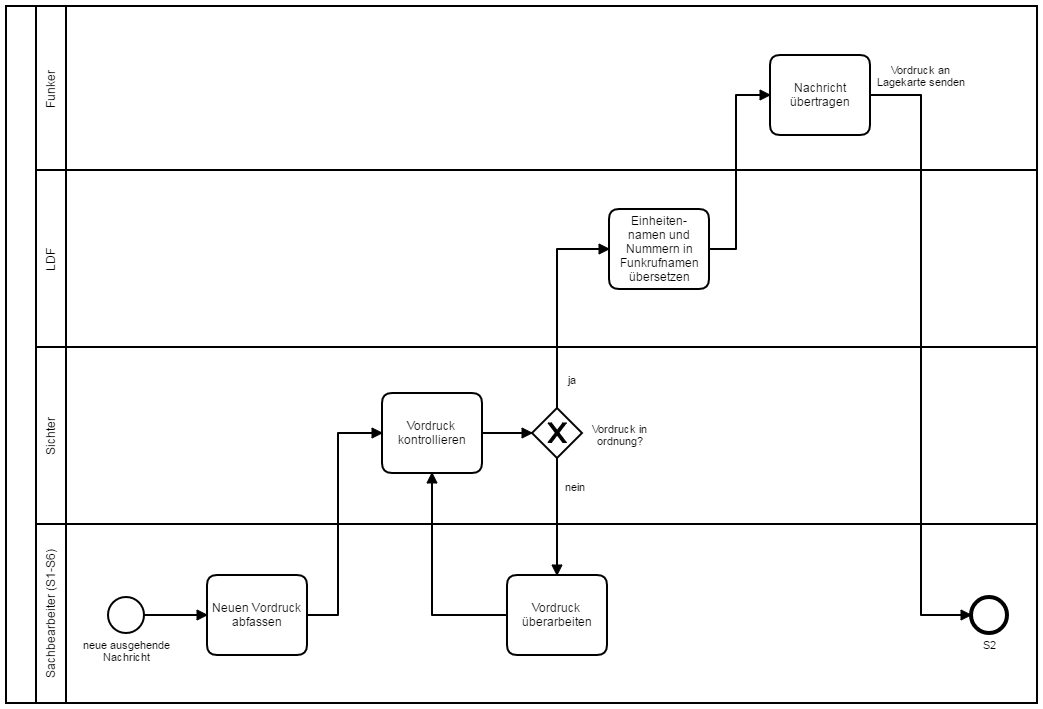
\includegraphics[width=0.95\linewidth]{ausgehend.png}
\end{figure} Ein Sachbearbeiter erhält eine neue ausgehende Nachricht und fasst einen neuen Vordruck ab. Dieser Vordruck wird von einem Sichter kontrolliert und an den LDF übermittelt. Der LDF übersetzt die Einheitennamen und Nummern in Funkrufnamen bevor der Vordruck an den Funker zur Übertragung weitergeleitet wird. Im Anschluss daran erhält Sachbearbeiter S2 (Lagekarte) den Vordruck, womit der Vorgang abgeschlossen wird.

\newpage
\subsection{/LC0200/ Eingehende Nachrichten} 
\begin{figure}[htpb]
	\centering
	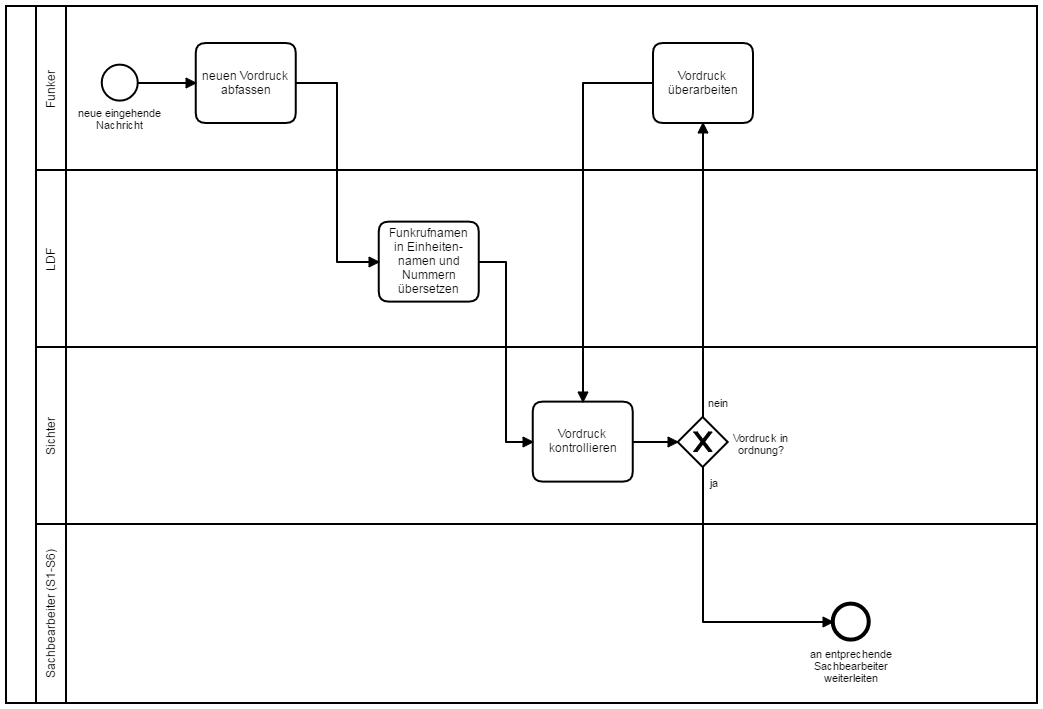
\includegraphics[width=0.95\linewidth]{eingehend.png}
\end{figure} Ein Funker erhält eine neue eingehende Nachricht und fasst einen neuen Vordruck ab. Der LDF übersetzt die Funkrufnamen in Einheitennamen und Nummern bevor der Vordruck zur Kontrolle an einen Sichter gesendet wird. Anschließend wird der Vordruck an die entprechenden Sachbearbeiter übermittelt

\subsection{/LC0300/ Kontrolle durch Sichter}
Ein Sichter erhält einen Vordruck zur Kontrolle und stuft diesen als unzureichend ein. Der Vordruck wird dann zurück an den Verfasser gesendet, welcher diesen überarbeitet und zur erneuten Kontrolle an den Sichter schickt. Wird ein Vordruck vom Sichter erfolgreich abgenommen durchläuft er den weiteren Workflow.

\subsection{/LC0400/ Ausdrucken eines Vordruckes}
Das System bietet dem Nutzer die Möglichkeit, sich einen verfassten oder erhaltenen Vordruck anzuschauen und auszudrucken.